% Signals and Systems (ETH Zurich, HS26, Dr. A. Carron) -- exam cheat sheet
% Format: A4 landscape, 4 columns, ETH-style section bars (after ZF strubma/bmicha).
% Page 1 = front, page 2 = back. Theory only (no worked examples). Weeks 1-7 so far.
\RequirePackage{fix-cm}
\documentclass[a4paper,landscape]{article}
\usepackage[a4paper,landscape,margin=3mm,top=2.8mm,bottom=3mm]{geometry}
\usepackage{amsmath,amssymb,mathtools}
\usepackage{multicol}
\usepackage[dvipsnames,table]{xcolor}
\usepackage{enumitem}
\usepackage{array,tabularx,booktabs}
\usepackage{tikz}
\usetikzlibrary{arrows.meta,positioning}

\renewcommand{\familydefault}{\sfdefault}
\pagestyle{empty}
\setlength{\parindent}{0pt}
\setlength{\parskip}{0pt}
\setlength{\columnsep}{2.2mm}
\setlength{\columnseprule}{0.25pt}
\setlength{\arraycolsep}{1.2pt}
\setlength{\tabcolsep}{1.4pt}
\renewcommand{\arraystretch}{0.9}
\setlist{nosep,leftmargin=5pt,labelsep=1.5pt,itemsep=0pt,topsep=0pt,partopsep=0pt}
\setlist[itemize]{label=$\bullet$}
\medmuskip=1.6mu plus 1mu minus 1.6mu
\thickmuskip=2.4mu plus 2mu minus 2mu
\thinmuskip=1.3mu
\newcolumntype{Y}{>{\raggedright\arraybackslash}X}
\newcolumntype{C}{@{\hspace{0.5pt}}>{\centering\arraybackslash}p{2.1mm}@{\hspace{0.4pt}}}

\definecolor{secblue}{HTML}{3C78D8}
\definecolor{subblue}{HTML}{D2E2F8}
\definecolor{warnred}{HTML}{B3261E}
\setlength{\fboxsep}{0.8pt}
\newcommand{\sect}[1]{\par\vspace{1pt}\noindent\colorbox{secblue}{\parbox{\dimexpr\linewidth-2\fboxsep}{\color{white}\bfseries\fontsize{6.8}{7.6}\selectfont\strut #1}}\par\vspace{0.4pt}}
\newcommand{\sub}[1]{\par\vspace{0.6pt}\noindent\colorbox{subblue}{\parbox{\dimexpr\linewidth-2\fboxsep}{\bfseries\strut #1}}\par\vspace{0.2pt}}
\newcommand{\warn}[1]{{\color{warnred}\textbf{!}\,#1}}
\newcommand{\up}[1]{\underset{\uparrow}{#1}}
\newcommand{\T}{^{\!\top}}
\newcommand{\bx}[1]{\fbox{$\textstyle #1$}}
\newcommand{\cm}{\ensuremath{\checkmark}}
\newcommand{\xm}{\ensuremath{\times}}
\newcommand{\eqc}[1]{\par\vspace{0.2pt}\centerline{$#1$}\par\vspace{0.2pt}}

\DeclareMathSizes{6.5}{6.5}{4.7}{3.8}
\begin{document}
\fontsize{6.5}{7.3}\selectfont\raggedright
\setlength{\abovedisplayskip}{0.6pt}\setlength{\belowdisplayskip}{0.6pt}
\setlength{\abovedisplayshortskip}{0.3pt}\setlength{\belowdisplayshortskip}{0.3pt}
\setlength{\jot}{0.2pt}
\begin{multicols*}{4}
{\fontsize{5.2}{5.8}\selectfont Signals \& Systems, ETH HS26 $\cdot$ W1--7 $\cdot$ $u$ input, $y$ output, $s[n]$ unit step, $h$ impulse response\par}

% =====================================================================
\sect{Math Toolbox}
$\sum_{k\ge0}a^k=\frac1{1-a}\,(|a|{<}1)$, $\sum_{k=0}^{N-1}a^k=\frac{1-a^N}{1-a}$, $\sum_{k\ge0}ka^k=\frac{a}{(1-a)^2}$.
$z=a{+}jb=re^{j\theta}$, $e^{j\theta}=\cos\theta+j\sin\theta$, $\cos\theta=\frac{e^{j\theta}+e^{-j\theta}}2$, $\sin\theta=\frac{e^{j\theta}-e^{-j\theta}}{2j}$, $\frac1z=\frac{\bar z}{|z|^2}$; $|z_1z_2|=|z_1||z_2|$, $\angle z_1z_2=\angle z_1{+}\angle z_2$, $\angle\frac{z_1}{z_2}=\angle z_1{-}\angle z_2$.
\textbf{Angle} from $+$Re axis, ccw: $\angle1{=}0$, $\angle j{=}\frac\pi2$, $\angle({-}1){=}\pi$, $\angle(1{+}j){=}\frac\pi4$; 2nd quadrant ($a{<}0{<}b$): $\angle(a{+}jb)=\pi-\arctan\frac{b}{|a|}$. Real coeff.\ $\Rightarrow$ complex roots in conj.\ pairs.
$\begin{bsmallmatrix}a&b\\c&d\end{bsmallmatrix}^{-1}{=}\frac{1}{ad-bc}\begin{bsmallmatrix}d&-b\\-c&a\end{bsmallmatrix}$, $\det(zI{-}A)=z^2-\mathrm{tr}A\,z+\det A$; triangular: eig.\ = diagonal.
$z^2-2\alpha z+c=0$: $z=\alpha\pm\sqrt{\alpha^2-c}$; complex $\Rightarrow|z|=\sqrt c$.
$1\pm e^{-j\Omega}=e^{-j\Omega/2}(e^{j\Omega/2}\pm e^{-j\Omega/2})$: $1{-}e^{-j\Omega}=2j\sin\frac\Omega2e^{-j\Omega/2}$, $1{+}e^{-j\Omega}=2\cos\frac\Omega2e^{-j\Omega/2}$.

% =====================================================================
\sect{W1 \ Signals}
CT $x(t)$, $t\in\mathbb R$; DT $x[n]$, $n\in\mathbb Z$ (sequence); $\{x[n]\}$ whole signal. Sequence notation: $\uparrow$ marks $n{=}0$, unlisted samples $=0$ (count from the arrow).\\
$\alpha x[n]$ scaling; \ $x[n{-}k]$ ($k{>}0$) \textbf{delay} = shift \textbf{right}; \ $x[n{+}k]$ \textbf{advance} = shift \textbf{left}; \ $x[-n]$ flip about $n{=}0$ ($x[0]$ stays). Locate a sample: set argument $=$ its index.
\textbf{Combined} (read inside out): $x[-n{+}k]=x[-(n{-}k)]$: flip, then shift right by $k$; value at $n$ is $x[k-n]$.\\
$\delta[n]{=}1$ iff $n{=}0$ (else 0); $s[n]{=}1$ iff $n\ge0$. \ $\bx{s[n]=\sum_{k\le n}\delta[k],\ \delta[n]=s[n]-s[n{-}1]}$\\
\textbf{Impulse decomposition} $\bx{x[n]=\sum_kx[k]\,\delta[n-k]}$ (one term per nonzero sample). Sifting: $x[n]\delta[n{-}k]=x[k]\delta[n{-}k]$.
\textbf{Causal signal}: $x[n]{=}0\ \forall n{<}0$. \textbf{Bounded}: $|x[n]|\le M<\infty\ \forall n$.

% =====================================================================
\sect{W1 \ System Properties}
System $G$: $u\mapsto y=Gu$. A property holds for \emph{all} inputs: prove with the definition, disprove with \emph{one} counterexample.\\
\begin{tabularx}{\linewidth}{@{}lY@{}}
Memoryless & $y[n]$ depends only on $u[n]$ (any other index $\Rightarrow$ memory)\\
Causal & only on $u[k]$, $k\le n$ (index $>n$, or $u[-n]$ $\Rightarrow$ non-causal)\\
Linear & $G\{\alpha_1u_1{+}\alpha_2u_2\}=\alpha_1Gu_1{+}\alpha_2Gu_2$ $\forall u_i,\alpha_i$; implies $0\mapsto0$\\
Time-inv. & $u_1[n{-}k]\mapsto y_1[n{-}k]$ $\forall k$: compute $G\{u_1[n{-}k]\}$, compare with $y_1[n{-}k]$ (replace \emph{every} $n$ by $n{-}k$)\\
BIBO stable & $|u[n]|{\le}1\ \forall n\Rightarrow|y[n]|{\le}M{<}\infty$; disprove with one bounded $u$ giving unbounded $y$ (try $u{=}s$)
\end{tabularx}
\textbf{Linearity fails:} constant offset (affine $\ne$ linear), $u^2$, $|u|$, $\cos u$, products $u[n]u[n{-}1]$. \textbf{TI fails:} explicit $n$ in coefficients ($n\,u[n]$, $g[n]u[n]$), time scaling $u[2n]$, reversal $u[-n]$ (delayed input comes out advanced). $g[n]u[n]$ is linear for every fixed $g$. Accumulator $\sum_{k\le n}u[k]$ and $y[n]{=}ay[n{-}1]{+}u[n]$, $|a|{\ge}1$: unstable. Bounded nonlinearities ($\cos u$) are stable. Linear but not TI: response to $\delta$ does not give response to shifted inputs. Physical systems are causal; non-causal = offline processing.

% =====================================================================
\sect{W2 \ Impulse Response \& Convolution}
$\bx{h[n]:=G\{\delta[n]\}}$. LTI shift rule: $\delta[n{-}k]\mapsto h[n{-}k]$ (TI), $c\,\delta[n{-}k]\mapsto c\,h[n{-}k]$ (L). For LTI, $h$ determines the output for every input; not for non-LTI.
\eqc{\bx{y[n]=(u*h)[n]=\textstyle\sum_ku[k]\,h[n-k]=\sum_kh[k]\,u[n-k]}}
Needs L \emph{and} TI. Flip \& slide (either signal may be flipped), or $y[n]=\sum_{i+j=n}u[i]h[j]$ (polynomial product). \textbf{Length} $L_y=L_u+L_h-1$; first index $=n_{u,0}+n_{h,0}$, last $=$ sum of last indices. Check: $\sum_ny=\sum u\cdot\sum h$.\\
\textbf{Properties:} commutative, associative, distributive; identity $u*\delta=u$; $u*\delta[n{-}k]=u[n{-}k]$; \warn{$u*h\ne u\cdot h$}. \textbf{Series} $\Rightarrow h_1*h_2$ (LTI blocks may be interchanged; not for non-LTI), \textbf{parallel} $\Rightarrow h_1+h_2$, direct path $\Rightarrow+\delta$.
\textbf{Deconvolution} ($h[0]{\ne}0$): $u[n]=(y[n]-\sum_{k\ge1}h[k]u[n{-}k])/h[0]$ recursively.\\
\textbf{Step response} $\bx{r[n]=(h*s)[n]=\sum_{k\le n}h[k]},\ \bx{h[n]=r[n]-r[n{-}1]}$ (either one characterizes the LTI system). Stable: $r[\infty]=\sum_kh[k]=H(1)$.
\sub{Causality, Stability, FIR/IIR (LTI)}
$\bx{\text{causal}\iff h[n]=0\ \forall n<0}$ (nonzero $h[m]$, $m{<}0$, weighs the future input $u[n{-}m]$). Causal \emph{system} $\ne$ causal \emph{signal}. Memoryless $\iff h=c\,\delta$.
$\bx{\text{BIBO stable}\iff\sum_k|h[k]|<\infty}$, since $|y[n]|\le\sum_k|h[k]|\,\max|u|$. $\alpha^ns[n]$: $\sum=\frac1{1-|\alpha|}$, stable iff $|\alpha|{<}1$.
\warn{Traps:} causal $\not\Rightarrow$ stable; bounded $h$ $\not\Rightarrow$ stable ($s[n]$); $h\to0$ $\not\Rightarrow$ stable ($\frac1{n+1}s[n]$, harmonic sum); left-sided $a^n$ ($n{\le}0$) with $|a|{>}1$ is stable (support decides, not base); an unstable block can be cancelled in a cascade ($s*(\delta-\delta[n{-}1])=\delta$): judge the overall $h$.
\textbf{FIR}: finitely many $h[n]{\ne}0$ $\Rightarrow$ always stable. \textbf{IIR}: infinitely many (stable or not).
Feedback $y[n]=u[n]+\alpha y[n{-}D]$: $h=\sum_{k\ge0}\alpha^k\delta[n{-}kD]$, IIR, stable iff $|\alpha|{<}1$.

% =====================================================================
\sect{W3 \ System Representations}
$h[n]$ (analysis) $\cdot$ LCCDE (real-time/DSP) $\cdot$ state space (simulation, design). Fixed-memory real time: recursion \& SS yes; convolution with IIR $h$ no.
\sub{LCCDE \& State Space}
$\bx{\sum_{k=0}^Na_ky[n{-}k]=\sum_{k=0}^Mb_ku[n{-}k]}$, $a_0{\ne}0$, LTI by definition, order $N$ = largest output delay. Recursion: $y[n]=\frac1{a_0}(\sum_{k=0}^Mb_ku[n{-}k]-\sum_{k=1}^Na_ky[n{-}k])$.
\textbf{LCCDE$\to h$:} iterate with $u{=}\delta$, $y[n]{=}0$ for $n{<}0$. \warn{$y[n]-a\,y[n{-}1]$ has ratio $+a$.} \textbf{$h\to$ LCCDE:} FIR: $b_k{=}h[k]$; sum of geometric terms: via $H(z)$.
\eqc{\bx{q[n{+}1]=Aq[n]+Bu[n],\quad y[n]=Cq[n]+Du[n]}}
$A_{N\times N}$, $B_{N\times1}$, $C_{1\times N}$, $D$ = feedthrough (instant $u\to y$). \textbf{State} = everything from the past that still affects the future: equal $q[n]$ + equal future input $\Rightarrow$ equal future output. Dimension $N$ = order; inputs are not states; one state per stored value / energy store.\\
\textbf{SS$\to h$} ($q[0]{=}0$, $q[n]{=}A^{n-1}B$): $\bx{h=\{\up D,CB,CAB,CA^2B,\dots\}}$, $h[n]=CA^{n-1}B$ ($n{\ge}1$). \warn{$h[0]=D$, not $CB$}; $D{=}0\Rightarrow$ response 1 sample late. Initial state adds free response $CA^nq[0]$.\\
\textbf{LCCDE$\to$SS} (companion form, $a_0{=}1$, RHS $b_0u[n]$, $q=[y[n{-}N],..,y[n{-}1]]\T$):
$A=\begin{bsmallmatrix}0&1&0\\0&0&1\\-a_3&-a_2&-a_1\end{bsmallmatrix}$, $B=\begin{bsmallmatrix}0\\0\\b_0\end{bsmallmatrix}$ (shown $N{=}3$), $C=[-a_N\cdots-a_1]$, $D=b_0$.
Delayed inputs ($M{\le}N$): same $A$, $B=[0..0\,1]\T$, $C=[b_N{-}a_Nb_0,..,b_1{-}a_1b_0]$, $D=b_0$; or put past inputs into the state.\\
\textbf{SS$\to$LCCDE}: eliminate $q$ (equation one step earlier, subtract) or via $H(z)$; scalar: $y[n]-Ay[n{-}1]=Du[n]+(CB-AD)u[n{-}1]$.
\textbf{Realizations not unique:} $q'=Tq$: $(TAT^{-1},TB,CT^{-1},D)$ gives the same $h$. Compare realizations via $h$ or $H(z)$, never entrywise.
\sub{CT State Space \& Linearization}
$\bx{\dot q=A_cq+B_cu,\ y=C_cq+D_cu}$. Build: rows $\dot q_1{=}q_2$ (definitions), last row = physical law solved for the highest derivative. $m\ddot p{+}c\dot p{+}kp{=}F$, $q{=}[p,\dot p]\T$: $A_c{=}\begin{bsmallmatrix}0&1\\-\frac km&-\frac cm\end{bsmallmatrix}$, $B_c{=}\begin{bsmallmatrix}0\\\frac1m\end{bsmallmatrix}$.\\
\textbf{1.} Equilibrium $(q_e,u_e)$: $\bx{f(q_e,u_e)=0}$, $y_e=h(q_e,u_e)$; $u_e{\ne}0$ allowed, several may exist, $\partial f/\partial q{=}0$ not required.
\textbf{2.} Jacobians evaluated at $(q_e,u_e)$ (row = equation, column = variable): $A_c{=}\frac{\partial f}{\partial q}|_e$, $B_c{=}\frac{\partial f}{\partial u}|_e$, $C_c{=}\frac{\partial h}{\partial q}|_e$, $D_c{=}\frac{\partial h}{\partial u}|_e$.
\textbf{3.} $\bx{\Delta\dot q=A_c\Delta q+B_c\Delta u,\ \Delta y=C_c\Delta q+D_c\Delta u}$, $\Delta q=q-q_e$, $\Delta u=u-u_e$, $\Delta y=y-y_e$. Constant matrices $\Rightarrow$ LTI; valid only for small deviations (neglected higher-order terms grow faster). \warn{No $q$, $\sqrt q$, $\sin q$ left in the matrices.} One linear model per equilibrium.

% =====================================================================
\sect{W4 \ Sampling \& Discretization}
\textbf{Sampler} $S$ (CT$\to$DT): $\bx{x[n]=x(nT_s)}$, $f_s{=}\frac1{T_s}$; values between samples lost. \textbf{ZOH} $H$ (DT$\to$CT): $\bx{x(t)=x[n],\ t\in[nT_s,(n{+}1)T_s)}$, staircase (linear interpolation would be first-order hold). $S\circ H=\mathrm{id}$, $H\circ S\ne\mathrm{id}$.
\centerline{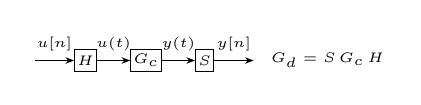
\begin{tikzpicture}[font=\tiny,node distance=4.2mm,>={Stealth[length=1.1mm]},b/.style={draw,minimum height=2.8mm,inner sep=1pt}]
\node[b](H){$H$};\node[b,right=of H](G){$G_c$};\node[b,right=of G](S){$S$};
\draw[->](H.west)++(-5mm,0)--node[above]{$u[n]$}(H.west);\draw[->](H)--node[above]{$u(t)$}(G);\draw[->](G)--node[above]{$y(t)$}(S);\draw[->](S.east)--node[above]{$y[n]$}++(5mm,0);
\node[right=6mm of S]{$G_d=S\,G_c\,H$};
\end{tikzpicture}}
Composition read right to left; $u[n],y[n]$ DT, $u(t),y(t)$ CT; under ZOH $u(t)$ constant per interval (no averaging of $u[n],u[n{+}1]$). Pure delay $kT_s{<}\tau{\le}(k{+}1)T_s\Rightarrow y[n]=u[n{-}k{-}1]$ (rounded up).
\sub{Euler \& Exact Discretization}
\textbf{Euler} $\dot q\approx\frac{q(t+T_s)-q(t)}{T_s}$: $\bx{A_d=I+T_sA_c,\ B_d=T_sB_c,\ C_d=C_c,\ D_d=D_c}$; output eq.\ has no derivative $\Rightarrow$ $C,D$ unchanged. Error $\mathcal O(T_s^2)$/step.
Stable iff $|1+T_s\lambda_i(A_c)|<1$; scalar $a{<}0$: $\bx{T_s<2/|a|}$, monotone iff $T_s<1/|a|$; for $\frac1{|a|}{<}T_s{<}\frac2{|a|}$ decays with sign flips; beyond: growing alternation (stable CT model becomes unstable).\\
\textbf{Exact (ZOH)}: input held, augment $r=[q;u]$, $\dot r=Mr$:
$\bx{M=\begin{bsmallmatrix}A_c&B_c\\0&0\end{bsmallmatrix},\ e^{MT_s}=\begin{bsmallmatrix}A_d&B_d\\0&I\end{bsmallmatrix}}$, $A_d{=}e^{A_cT_s}$ (top-left), $B_d$ top-right ($=A_c^{-1}(A_d{-}I)B_c$), $C_d{=}C_c$, $D_d{=}D_c$.
Scalar: $\bx{a_d=e^{aT_s},\ b_d=\frac ba(e^{aT_s}-1)}$ ($a{=}0$: $b_d=bT_s$); $M^k=\begin{bsmallmatrix}a^k&a^{k-1}b\\0&0\end{bsmallmatrix}$. Eigenvalues $\lambda\mapsto e^{\lambda T_s}$, $|e^{\lambda T_s}|=e^{\mathrm{Re}\lambda T_s}$: stability kept for every $T_s$; stable 1st order $a_d\in(0,1)$. Exact at samples, inter-sample behaviour lost. Euler = exponential series truncated after linear term.\\
\begin{tabular}{@{}llll@{}}\toprule
&$A_d$&$B_d$&accuracy / stability\\\midrule
Euler & $I{+}T_sA_c$ & $T_sB_c$ & $\mathcal O(T_s^2)$; stable only for small $T_s$\\
Exact & $e^{A_cT_s}$ & top-right of $e^{MT_s}$ & exact at samples; always kept\\\bottomrule
\end{tabular}\\
Fast dynamics / large $T_s$ $\Rightarrow$ exact; slow dynamics \& small $T_s$ $\Rightarrow$ Euler OK.\\
$e^{At}=\sum\frac{(At)^k}{k!}$ (\emph{not} entrywise): diag $\mapsto$ diag$(e^{\lambda_it})$; nilpotent: series ends; $\begin{bsmallmatrix}\lambda&1\\0&\lambda\end{bsmallmatrix}\mapsto e^{\lambda t}\begin{bsmallmatrix}1&t\\0&1\end{bsmallmatrix}$; $\begin{bsmallmatrix}\sigma&\omega\\-\omega&\sigma\end{bsmallmatrix}\mapsto e^{\sigma t}\begin{bsmallmatrix}\cos\omega t&\sin\omega t\\-\sin\omega t&\cos\omega t\end{bsmallmatrix}$; $A{=}V\Lambda V^{-1}\Rightarrow Ve^{\Lambda t}V^{-1}$.
Integrator $\dot q{=}u$: $(1,T_s)$; double integrator $\dot p{=}v,\dot v{=}u$: $A_d{=}\begin{bsmallmatrix}1&T_s\\0&1\end{bsmallmatrix}$, $B_d{=}\begin{bsmallmatrix}T_s^2/2\\T_s\end{bsmallmatrix}$ (Euler misses $T_s^2/2$).

% =====================================================================
\sect{W5 \ The z-Transform \& z-Plane}
$z_0$ (number) $\to z_0^n$ (signal) $\to H(z_0)$ (eigenvalue, one number) $\to H(z)$ (function on ROC). \textbf{Eigenfunction:} $\bx{u=z_0^n\ \forall n\Rightarrow y=H(z_0)z_0^n}$, $H(z_0)=\sum_kh[k]z_0^{-k}$ ($z_0$ in ROC). $u\equiv1\Rightarrow y=H(1)$ (DC gain).
$z^n=r^ne^{j\theta n}$: $r$ envelope ($<1$ decay, $=1$ sustained, $>1$ growth), $\theta$ phase advance per sample.
\eqc{\bx{X(z)=\textstyle\sum_{n=-\infty}^{\infty}x[n]z^{-n}},\quad Y(z)=H(z)U(z)}
\textbf{ROC}: never contains poles; causal/right-sided $|z|{>}\max|p|$, left-sided $|z|{<}\min|p|$, two-sided annulus, causal FIR all $z{\ne}0$. Expression unique only with ROC or causality ($a^ns[n]$ and $-a^ns[-n{-}1]$ both $\frac z{z-a}$). \textbf{Any LTI: stable $\iff$ ROC $\ni$ unit circle.} Delays keep the ROC (except $c\,\delta$ loses $z{=}0$).\\
\begin{tabular}{@{}ll|ll@{}}
$x[n{-}k]$ & $z^{-k}X$ & $a^nx[n]$ & $X(z/a)$\\
$x[n{+}k]$ & $z^kX$ & $n\,x[n]$ & $-zX'(z)$\\
$u*h$ & $UH$ & $x[-n]$ & $X(1/z)$\\
$\delta[n{-}k]$ & $z^{-k}$ & $\sum_{k\le n}x[k]$ & $\frac z{z-1}X$\\
$a^ns[n]$ & $\bx{\frac z{z-a}},|z|{>}|a|$ & $s[n]$ & $\frac z{z-1}$\\
$a^{n-1}s[n{-}1]$ & $\frac1{z-a}$ & $na^ns[n]$ & $\frac{az}{(z-a)^2}$\\
$(n{+}1)a^ns[n]$ & $\frac{z^2}{(z-a)^2}$ & $ns[n]$ & $\frac{z}{(z-1)^2}$
\end{tabular}\\
$r^n\cos(\theta n)s[n]\leftrightarrow\frac{z(z-r\cos\theta)}{z^2-2r\cos\theta z+r^2}$, $r^n\sin(\theta n)s[n]\leftrightarrow\frac{r\sin\theta z}{z^2-2r\cos\theta z+r^2}$. IVT $x[0]{=}\lim_{z\to\infty}X$ (causal); FVT $x[\infty]{=}\lim_{z\to1}(z{-}1)X$ (if limit exists).
FIR: $H(z)=\sum_kh[k]z^{-k}$, all poles at $0$. A zero on the unit circle at angle $\theta$ annihilates $e^{j\theta n}$ (zero at 1: constants, at $-1$: $(-1)^n$).
\sub{Obtaining $H(z)$}
$\bx{H(z)=\frac{b_0+b_1z^{-1}+\dots+b_Mz^{-M}}{1+a_1z^{-1}+\dots+a_Nz^{-N}}}$ (zero IC, delay $\to z^{-k}$), then multiply by $z^{\max(N,M)}$. \warn{Move all $y$-terms to the left first (signs flip).}
$\bx{H(z)=C(zI-A)^{-1}B+D}$, $(zI{-}A)^{-1}=\frac{\mathrm{adj}(zI-A)}{\det(zI-A)}$: poles $\subseteq$ eig$(A)$ (an eigenvalue may cancel with a zero). Feedback $u=-Kq+d$: $A_K=A-BK$.
\sub{Poles, Modes, Partial Fractions}
$H=b_0z^{N-M}\frac{\prod(z-z_i)}{\prod(z-p_k)}$: zeros $\circ$ (numerator roots), poles $\times$ (denominator roots); $N{>}M$: zeros at $0$.
\textbf{PFE:} $\frac{H}z=\frac dz+\sum\frac{c_k}{z-p_k}$, $c_k=[(z{-}p_k)\frac Hz]_{z=p_k}$, $d=H(0)$:
\eqc{\bx{H=d+\textstyle\sum_k\frac{c_kz}{z-p_k}\Rightarrow h[n]=d\,\delta[n]+\sum_kc_kp_k^ns[n]}}
One mode $p_k^n$ per pole, weights $c_k$ from the numerator. Conj.\ pair: $c p^n+\bar c\bar p^n=2|c|r^n\cos(\theta n{+}\angle c)$. Double pole: $(n{+}1)p^n$ (input at a pole: bounded if $|p|{<}1$). Settling to a constant $\ne$ stable (pole at 1).
\sub{Stability \& Pole Placement}
$\bx{\text{causal LTI stable}\iff\text{all poles }|p_k|<1}$; SS: all $|\lambda(A)|{<}1$ suffices. Zeros irrelevant; coefficients $\ne$ poles (a coefficient $>1$ says nothing). 2nd order $z^2{+}a_1z{+}a_0$ stable $\iff|a_0|{<}1,\,|a_1|{<}1{+}a_0$.
$0{<}p{<}1$: smooth decay, never changes sign; $-1{<}p{<}0$: alternating decay; $re^{\pm j\theta}$, $r{<}1$: decaying oscillation; $|p|{=}1$: sustained (tone), $p{=}1$ constant persists (not BIBO); $|p|{>}1$: grows. Two real modes: fast one dies first. \textbf{Dominant mode} = largest $|p|$.\\
\centerline{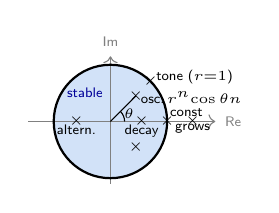
\begin{tikzpicture}[scale=0.72,font=\tiny]
\fill[subblue] (0,0) circle (1);
\draw[->,gray] (-1.45,0)--(1.85,0) node[right]{Re};\draw[->,gray] (0,-1.1)--(0,1.15) node[above]{Im};
\draw[thick] (0,0) circle (1);
\node[blue!60!black] at (-0.45,0.5) {stable};
\foreach \x/\y/\l/\pos in {0.55/0/decay/below, -0.6/0/altern./below, 1.45/0/grows/below}{\node at (\x,\y){$\times$};\node[\pos,inner sep=1pt] at (\x,\y){\l};}
\node at (0.45,0.45){$\times$};\node at (0.45,-0.45){$\times$};\node[right,inner sep=1pt] at (0.48,0.42){osc.\,$r^n\!\cos\theta n$};
\node at (1,0){$\times$};\node[above right,inner sep=0.5pt] at (1.02,0.05){const};
\node at (0.707,0.707){$\times$};\node[right,inner sep=1pt] at (0.75,0.78){tone ($r{=}1$)};
\draw (0,0)--(0.45,0.45); \draw (0.25,0) arc (0:45:0.25); \node at (0.33,0.13){$\theta$};
\end{tikzpicture}}
$\bx{(z{-}re^{j\theta})(z{-}re^{-j\theta})=z^2{-}2r\cos\theta z{+}r^2}$ $\Rightarrow$ $y[n]=2r\cos\theta\,y[n{-}1]-r^2y[n{-}2]+u[n]$ (numerator $z^2$).
Period $N_p$ samples: $\bx{\theta=2\pi/N_p}$; envelope $\to\varepsilon$ after $N$ samples: $\bx{r=\varepsilon^{1/N}}$; in Hz: $f=\theta f_s/2\pi$. Placement is in samples: changing $f_s$ for the same physical response changes $\theta$ and $r$ ($f_s/2$: $\theta\to2\theta$, $r\to r^2$). CT pole $\lambda$ $\leftrightarrow$ DT pole $e^{\lambda T_s}$.

% =====================================================================
\sect{W6 \ Frequency in DT \& Sampling}
$\Omega$ [rad/sample] = phase advance per sample; one cycle $=2\pi/\Omega$ samples; $\cos\Omega n=\mathrm{Re}\,e^{j\Omega n}$. \ $\bx{\Omega=\frac{2\pi f}{f_s}=\omega T_s,\ \ f=\frac{\Omega f_s}{2\pi}}$; $\frac{f}{f_s}$ = periods per sample. $\Omega$ alone has no Hz (needs $f_s$).\\
$e^{j(\Omega+2\pi)n}=e^{j\Omega n}\Rightarrow$ every distinct frequency in $\bx{\Omega\in(-\pi,\pi]}$ (axis is a circle). $\Omega{=}0$ constant; $\Omega{=}\pi$: $(-1)^n$, fastest = \textbf{Nyquist frequency} $f_s/2$. \warn{Reduce $\Omega$ mod $2\pi$ into $(-\pi,\pi]$ before comparing speeds}; closest to $\pi$ is fastest.\\
\textbf{Periodic} $\iff\bx{\Omega/2\pi=k/N\in\mathbb Q}$; period $N$ for $k/N$ irreducible (DT period is an integer, not $2\pi/\Omega$). Sum of periodic signals: period $=\mathrm{lcm}$ of periods.\\
\textbf{Decomposition/spectrum:} $x[n]=\sum_iA_i\cos(\Omega_in{+}\phi_i)$, $A\cos(\Omega n{+}\phi)=\frac A2e^{j(\Omega n+\phi)}+\frac A2e^{-j(\Omega n+\phi)}$: two lines at $\pm\Omega_i$, magnitude $\frac{A_i}2$ each; constant $c$: one line at $0$ of height $|c|$; $A\cos\pi n$: one line at $\pi$ of height $|A|$ ($\pm\pi$ coincide). Spectra add (no averaging); magnitude spectrum hides phase (sign $=$ phase shift $\pi$).
\sub{Aliasing, Folding, Nyquist}
\textbf{Aliases}: $\bx{\pm f+kf_s,\ k\in\mathbb Z}$ give identical samples ($f{\pm}kf_s$ alone misses the mirror branch). Branch $f{+}kf_s$: same phase; branch $-f{+}kf_s$: opposite phase (sine $\to$ $-$sine).
\textbf{Folding} (alias seen in $[0,\frac{f_s}2]$): (1) subtract multiples of $f_s$ into $(-\frac{f_s}2,\frac{f_s}2]$; (2) drop the sign. $\bx{f_a=|f-f_s\,\mathrm{round}(f/f_s)|}$. \warn{Fold with $f_s$, not $f_s/2$.} A frequency sweep is heard as a triangle:\\
\centerline{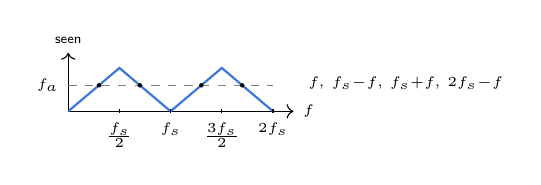
\begin{tikzpicture}[x=6.5mm,y=5.5mm,font=\tiny]
\draw[->] (0,0)--(4.4,0) node[right]{$f$};\draw[->] (0,0)--(0,1.35) node[above]{seen};
\draw[thick,secblue] (0,0)--(1,1)--(2,0)--(3,1)--(4,0);
\foreach \x/\l in {1/{\frac{f_s}2},2/{f_s},3/{\frac{3f_s}2},4/{2f_s}}{\draw (\x,0.05)--(\x,-0.05) node[below]{$\l$};}
\draw[dashed,gray] (0,0.6)--(4,0.6); \node[left] at (0,0.6){$f_a$};
\foreach \x in {0.6,1.4,2.6,3.4}{\fill (\x,0.6) circle (0.8pt);}
\node[right] at (4.5,0.65){$f,\,f_s{-}f,\,f_s{+}f,\,2f_s{-}f$};
\end{tikzpicture}}
\textbf{Nyquist:} samples determine the signal uniquely $\iff\bx{f_s>2f_{\max}}$ (strict: $\sin$ at exactly $f_s/2$ gives all-zero samples). Content above $f_s/2$ is \emph{not} removed: it folds onto genuine content as false tones; aliasing cannot be undone after sampling (a digital filter would also remove the genuine content there).
\textbf{Anti-aliasing filter}: CT low-pass \emph{before} the sampler, cutoff $f_c\approx f_{\max}$ of interest; real filters roll off gradually $\Rightarrow$ place $f_s/2$ above the transition band (margin). Disturbances \emph{inside} the band (e.g.\ 50\,Hz hum below $f_c$) pass and are not aliased: need a separate filter; raising $f_s$ does not help them. Choosing $f_s$: $f_{\max}\to f_c\to f_s>2f_c$ + margin.

% =====================================================================
\sect{W7 \ DTFT \& Frequency Response}
\eqc{\bx{X(\Omega):=X(z)\big|_{z=e^{j\Omega}}=\textstyle\sum_{n=-\infty}^{\infty}x[n]\,e^{-j\Omega n}}}
DTFT = z-transform on the unit circle; frequency $\Omega$ = angle of the point $e^{j\Omega}$: $\Omega{=}0$ DC ($z{=}1$), $\frac\pi2$ ($z{=}j$), $\pi$ Nyquist ($z{=}{-}1$). Of a signal: \textbf{spectrum}; of $h$: \textbf{frequency response} $H(\Omega)$. Complex: $X(\Omega)=|X(\Omega)|e^{j\angle X(\Omega)}$ (magnitude, phase). Periodic in $\Omega$ with period $2\pi$.\\
\textbf{Existence:} sum converges for every absolutely summable $x$ (every finite-length signal). Sinusoids/steps: not summable, DTFT only in a generalized sense. Causal rational $H$:
\eqc{\bx{\text{unit circle}\subset\text{ROC}\iff\text{poles inside}\iff\text{stable}\iff\textstyle\sum|h|<\infty}} frequency response exists iff stable; unstable systems (poles on/outside circle, e.g.\ $s[n]$, $(-1)^n$, $2^ns[n]$) have none.\\
\textbf{Real signals:} $\bx{X(-\Omega)=X(\Omega)^*}$: $|X|$ even, $\angle X$ odd $\Rightarrow$ plots over $[0,\pi]$ suffice (same for real $h$).
\sub{Computing \& Geometric Evaluation}
At $z=e^{j\Omega}$ evaluate numerator and denominator (two complex numbers): $\bx{|H(\Omega)|=\frac{|\mathrm{num}|}{|\mathrm{den}|},\ \angle H(\Omega)=\angle\mathrm{num}-\angle\mathrm{den}}$. On a zero: $H{=}0$, phase undefined.
\eqc{\bx{|H(\Omega)|=|b_0|\,\frac{\prod_i|e^{j\Omega}-z_i|}{\prod_k|e^{j\Omega}-p_k|}=|b_0|\frac{\prod\text{dist.\ to zeros}}{\prod\text{dist.\ to poles}}}}
$\angle H(\Omega)=\angle b_0+\sum\angle(e^{j\Omega}{-}z_i)-\sum\angle(e^{j\Omega}{-}p_k)$. Poles/zeros at the origin: distance 1, affect phase only.
\begin{itemize}
\item \textbf{Zero on the unit circle} at angle $\theta$: $|H(\theta)|=0$ (notch, frequency removed).
\item \textbf{Pole near the unit circle}: peak near its angle; closer $\Rightarrow$ higher and narrower.
\item \textbf{Pole close to a zero}: distances nearly equal $\Rightarrow$ $|H|$ almost constant away from the pair.
\item Near a pole large, on a zero vanishes; evaluation point moving away from the poles $\Rightarrow$ $|H|$ decreases.
\item 1st order $H=\frac{z}{z-a}=\frac1{1-ae^{-j\Omega}}$: $|H(0)|=\frac1{|1-a|}$, $|H(\pi)|=\frac1{|1+a|}$; $a{>}0$ low-pass, $a{<}0$ high-pass; $|H|^2=\frac1{1-2a\cos\Omega+a^2}$.
\item Delay $z^{-k}$: $H=e^{-jk\Omega}$, $|H|=1$ (0\,dB), linear phase $-k\Omega$. First difference $1{-}z^{-1}$: $H=2\sin\frac\Omega2\,e^{j(\frac\pi2-\frac\Omega2)}$ (high-pass, $H(0){=}0$, linear phase). $1{+}z^{-1}$: $2\cos\frac\Omega2e^{-j\Omega/2}$ (low-pass, $H(\pi){=}0$).
\end{itemize}
\sub{Bode Plot}
Over $\Omega\in[0,\pi]$: magnitude $\bx{20\log_{10}|H(\Omega)|}$ [dB] and phase $\angle H(\Omega)$ [rad]. Compute $H$ at selected frequencies (geometrically or from the formula), convert, connect.
$|H|\!:\ 10\to+20$, $2\to+6$, $\sqrt2\to+3$, $1\to0$, $0.707\to-3$, $0.5\to-6$, $0.1\to-20$, $0.01\to-40$, $0\to-\infty$\,dB; $|H|=10^{\text{dB}/20}$; every $-20$\,dB divides by 10; products of factors $\Rightarrow$ dB add.
\sub{Response to Sinusoids}
Stable LTI, $u[n]=e^{j\Omega_0n}$ for all $n$: $\bx{y[n]=H(\Omega_0)\,e^{j\Omega_0n}}$ (eigenfunction, one complex multiplication).
Real $h$: \ $\bx{u=A\cos(\Omega_0n{+}\phi)\Rightarrow y=A\,|H(\Omega_0)|\cos(\Omega_0n{+}\phi{+}\angle H(\Omega_0))}$:
same frequency, amplitude scaled by $|H(\Omega_0)|$, phase shifted by $\angle H(\Omega_0)$ (delay of $-\angle H/\Omega_0$ samples). Sums of sinusoids: apply per component (superposition). Constant input $c$: $y=cH(0)$.
\textbf{Steady state vs.\ transient:} for $u=\cos(\Omega_0n)s[n]$ (switched on at $n{=}0$) and a stable system: $y[n]\to|H(\Omega_0)|\cos(\Omega_0n{+}\angle H(\Omega_0))$ as $n\to\infty$; the difference (transient) consists of the decaying modes $p_k^n$. Formula exact only if input applied for all $n$.
A system that creates new frequencies (harmonics, distortion) is \emph{not} LTI; LTI systems only scale and shift each frequency.
\end{multicols*}
\end{document}
